\documentclass[]{beamer}
\usepackage{scalefnt}
\usepackage{graphicx}
\usepackage{tikz}
% Class options include: notes, notesonly, handout, trans,
%                        hidesubsections, shadesubsections,
%                        inrow, blue, red, grey, brown

% Theme for beamer presentation.
\usetheme{Copenhagen}
\usecolortheme{beaver}
% Other themes include: beamerthemebars, beamerthemelined, 
%                       beamerthemetree, beamerthemetreebars  
\setbeamertemplate{headline}{}

\title{\textbf{HQL} - \textsc{Hiperfit} Quant Library}    % Enter your title between curly braces
\author[shortname]{Johan Astborg \inst{1} \and Andreas Bock \inst{2}}
\institute[shortinst]{\inst{1} Lund University \and %
                      \inst{2} University of Copenhagen}
\date{\today}

\begin{document}

% Creates title page of slide show using above information
%\section[Outline]{}
\begin{frame}
  \titlepage
\end{frame}
\note{Talk for 30 minutes} % Add notes to yourself that will be displayed when
                           % typeset with the notes or notesonly class options


% Creates table of contents slide incorporating
% all \section and \subsection commands
\begin{frame}{Outline}
  \tableofcontents
\end{frame}

\section{Introduction}

\subsection{Problem statement}
\begin{frame}
  \frametitle{Introducing HQL}   % Insert frame title between curly braces
  \begin{block}{Open-source library for quantitative finance}
  \begin{itemize}
    \item Portfolio Management
    \item Pricing Utilities
    \item Haskell port of Sinan Gabel's \texttt{DerivativesExpert}
  \end{itemize}
  \end{block}
\end{frame}
\note[enumerate]       % Add notes to yourself that will be displayed when
{                      % typeset with the notes or notesonly class options 
}

\begin{frame}{Fixed Income}
    \begin{block}{Bonds}
    \begin{itemize}
       \item A contract that promises a future payment
       \item Either fixed or floating interest rate
       \item Priced using closed-form solutions
    \end{itemize}
    \end{block}
\end{frame}
%\note{Speak clearly}  % Add notes to yourself that will be displayed when
                       % typeset with the notes or notesonly class options

\section{\textsc{HQL} Demo}
\begin{frame}
\frametitle{Overview of the \textsc{HQL} library}
        \includegraphics[scale=0.25]{images/classhier.png}
\end{frame}

\begin{frame}
\frametitle{\textsc{HQL} Demo}
    \begin{block}{Objective: Buying me a house}
      \begin{itemize}
        \item Low-income, sensitive to variable cost
        \item Offer: serial loan from Swedbank
        \item How do I assess their offer?
        \item On what grounds should I accept?
      \end{itemize}
    \end{block}
    \begin{center}
        Use \textsc{HQL}!
    \end{center}
\end{frame}

% Model a serial in Haskell
% Fixed repayments sounds attractive
% Show repayments graphically
% Show cashflow graphically
% Explain coupons
% Accept defeat

\begin{frame}
\frametitle{\textsc{HQL} Demo}
    \begin{block}{Objective: Buying me a house}
      \begin{itemize}
        \item Second offer: annuity loan from Nordea
      \end{itemize}
    \end{block}
\end{frame}

% Model an annuity in Haskell
% Fixed payments! YUSS!!!
% Show repayments graphically
% Show cashflow graphically
% Victory!

\begin{frame}{Comparing cashflows}
{\scalefont{0.5}
\begin{figure}[!h]
\begin{center}
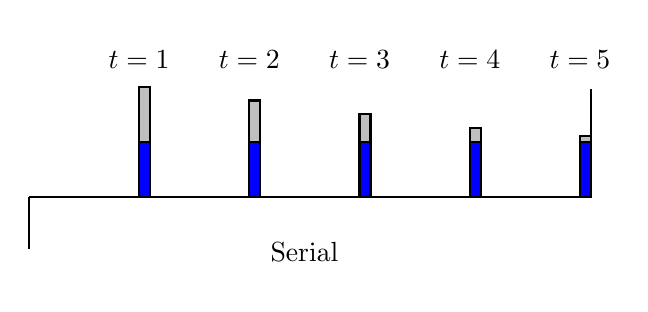
\begin{tikzpicture}[-,shorten >=1pt,auto,node distance=1.5cm,thick,minimum size=0.8cm,main node/.style={circle,draw=red,very thick},scale=0.7]
\tikzstyle{selected edge} = [draw,line width=6pt,-,blue!30]
%\tikzstyle{every node}=[font \small]

\coordinate (belowstart) at (0,-1);
\coordinate (start) at (0,0);
\coordinate (stop) at (10.2,0);
\coordinate (abovestop) at (10.2,2);
\draw (start) -- (stop);
\draw (start) -- (belowstart);
\draw (stop) -- (abovestop);

%\node at (0, -1.5) () {$t=0$};

\filldraw[draw=black, fill=blue] (2,0) rectangle node {} +(0.2,1);
\filldraw[draw=black, fill=lightgray]  (2,1) rectangle node {} +(0.2,1);
\node at (2, 2.5) () {$t=1$};

\filldraw[draw=black, fill=blue] (4,0) rectangle node {} +(0.2,1);
\filldraw[draw=black, fill=lightgray]  (4,1) rectangle node {} +(0.2,0.75);
\node at (4, 2.5) () {$t=2$};

\filldraw[draw=black, fill=blue] (6,0) rectangle node {} +(0.2,1);
\filldraw[draw=black, fill=lightgray]  (6,1) rectangle node {} +(0.2,0.5);
\node at (6, 2.5) () {$t=3$};
\node at (5, -1) () {\normalsize Serial};

\filldraw[draw=black, fill=blue] (8,0) rectangle node {} +(0.2,1);
\filldraw[draw=black, fill=lightgray]  (8,1) rectangle node {} +(0.2,0.25);
\node at (8, 2.5) () {$t=4$};

\filldraw[draw=black, fill=blue] (10,0) rectangle node {} +(0.2,1);
\filldraw[draw=black, fill=lightgray]  (10,1) rectangle node {} +(0.2,0.1);
\node at (10, 2.5) () {$t=5$};

% Legend
%\filldraw[draw=black, fill=blue] (7,-1) rectangle node {} +(0.2,0.2);
%\node at (8.3, -0.92) () {repayment};
%\filldraw[draw=black, fill=lightgray] (7,-1.5) rectangle node {} +(0.2,0.2);
%\node at (8, -1.44) () {coupon};
\end{tikzpicture}
\end{center}
\end{figure}

\vspace{-1cm}

\begin{figure}[h!]
\hspace{-0.7cm}
%\begin{center}
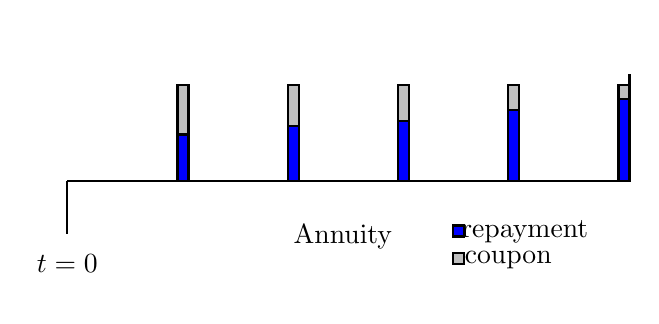
\begin{tikzpicture}[-,shorten >=1pt,auto,node distance=1.5cm,thick,minimum size=0.8cm,main node/.style={circle,draw=red,very thick}, scale=0.7]
\tikzstyle{selected edge} = [draw,line width=6pt,-,blue!30]

\coordinate (belowstart) at (0,-1);
\coordinate (start) at (0,0);
\coordinate (stop) at (10.2,0);
\coordinate (abovestop) at (10.2,2);
\draw (start) -- (stop);
\draw (start) -- (belowstart);
\draw (stop) -- (abovestop);

\node at (0, -1.5) () {$t=0$};

\filldraw[draw=black, fill=blue] (10,0) rectangle node {} +(0.2,1.5);
\filldraw[draw=black, fill=lightgray]  (10,1.5) rectangle node {} +(0.2,0.25);
%\node at (10, 2.5) () {$t=10$};

\filldraw[draw=black, fill=blue] (8,0) rectangle node {} +(0.2,1.3);
\filldraw[draw=black, fill=lightgray]  (8,1.3) rectangle node {} +(0.2,0.45);
%\node at (8, 2.5) () {$t=8$};

\filldraw[draw=black, fill=blue] (6,0) rectangle node {} +(0.2,1.1);
\filldraw[draw=black, fill=lightgray]  (6,1.1) rectangle node {} +(0.2,0.65);
%\node at (6, 2.5) () {$t=6$};
\node at (5, -1) () {\normalsize Annuity};

\filldraw[draw=black, fill=blue] (4,0) rectangle node {} +(0.2,1);
\filldraw[draw=black, fill=lightgray]  (4,1) rectangle node {} +(0.2,0.75);
%\node at (4, 2.5) () {$t=4$};

\filldraw[draw=black, fill=blue] (2,0) rectangle node {} +(0.2,0.85);
\filldraw[draw=black, fill=lightgray]  (2,0.85) rectangle node {} +(0.2,0.9);
%\node at (2, 2.5) () {$t=2$};

% Legend
\filldraw[draw=black, fill=blue] (7,-1) rectangle node {} +(0.2,0.2);
\node at (8.3, -0.92) () {repayment};

\filldraw[draw=black, fill=lightgray] (7,-1.5) rectangle node {} +(0.2,0.2);
\node at (8, -1.44) () {coupon};

\end{tikzpicture}
%\end{center}
\end{figure}}

\end{frame}


%\begin{frame}
%\frametitle{\textsc{HQL} Demo}
  %\begin{itemize}
    %\item Offer: annuity loan from Nordea
  %\end{itemize}
%\end{frame}

\begin{frame}
\frametitle{Present Value}
  \begin{block}{Pricing a future cashflow}
    \begin{equation}
      FV = N (1 + r) \Leftrightarrow N = \frac{FV}{1+r}
    \end{equation}
    \begin{itemize}
      \item $FV$ : Future Value
      \item $N$  : Amount invested
      \item $r$  : Interest Rate
    \end{itemize}
  \end{block}
\end{frame}

% Show audience the cashflow functionality of a SERIAL!

%% Present Value
\begin{frame}
\frametitle{Present Value}

  \begin{block}{Term structure}
  \begin{figure}[h!]
  \begin{tikzpicture}[-,shorten >=1pt,auto,node distance=1.5cm,thick,minimum size=0.8cm,main node/.style={circle,draw=red,very thick},scale=0.65]
  \tikzstyle{selected edge} = [draw,line width=6pt,-,blue!30]
  \coordinate (belowstart) at (0,-1);
  \coordinate (xaxis) at (10,0);
  \coordinate (origo) at (0,0);
  \coordinate (yaxis) at (0,5);

  % Draw axes
  \draw[->] (origo) -- (xaxis) node[right] {Time to maturity};
  \draw[->] (origo) -- (yaxis) node[above] {Annual rate};

  % "Normal" TS
  \draw[thick,draw=green] (0,0) parabola[bend at end] (10,5);
  \draw[dotted] (3,2.53) -- (3,0) node[below] {\text{ 3.5 years}};
  \draw[dotted] (3,2.53) -- (0,2.53) node[left] {2.4\%};

  \end{tikzpicture}
  \end{figure}
  \end{block}

\end{frame}

\begin{frame}
\frametitle{Bootstrapping a Term Structure}
\begin{itemize}
\item Create a term structure from market prices
\end{itemize}
\end{frame}

\section{Future Work}

\begin{frame}{Future Work}
  \begin{block}{Fixed Income}
    \begin{itemize}
      \item Mortgage-backed Bonds
      \item Floating Rate Bonds
    \end{itemize}
  \end{block}
            Interest Rate Derivatives\\
            Options
\end{frame}

%\begin{frame}{References}
%\bibliographystyle{apacite}  
%\bibliography{hql}  
%\end{frame}

\end{document}
